\documentclass[12pt,a4paper]{article}
\usepackage[utf8]{inputenc}
\usepackage[T1]{fontenc}
\usepackage{amsmath}
\usepackage{amsfonts}
\usepackage{amssymb}
\usepackage{graphicx}
\usepackage{physics}
\usepackage{cite}
\usepackage{caption}
\usepackage{subcaption}
\usepackage{hyperref}
\usepackage{comment}

\linespread{1.2}
\usepackage[a4paper,top=3cm,bottom=3cm,left=3cm,right=3cm]{geometry}

\title{On the ground state degeneracy of the Quantum Ising Model}
\author{}
\begin{document}
	\maketitle
\section{Goal}
We want to characterize the ground state of the 1D Quantum Ising Model, we will focus in particular on his symmetry properties and on the differences beetween the Classical and Quantum ground states.
\section{Some definitions}
The \textbf{2D Ising model} is a classical model composed of a 2D lattice of discrete variables $s_k$ such that  $s_k \in \{-1,1 \}$ and an Hamiltonian with two-sites and one-site terms:
\begin{equation}\label{eq:hamiltclass}
H_{CI}=-J\sum _{\langle i~j\rangle }s _{i}s _{j}-h\sum _{j}s _{j}
\end{equation}
The pointy brackets indicate nearest-neighbors. \\
The \textbf{Transverse-field Ising model} or \textbf{1D Quantum Ising model} \cite{sachdev_2011} is defined by a chain of spin-(1/2) variables interacting with an Hamiltonian of the form:
\begin{equation}\label{eq:hamiltqi}
H_{QI}=-J(\sum _{ l }\sigma_{l}^\parallel\sigma_{l+1}^\parallel+\lambda\sum _{l}\sigma_{l}^\perp)
\end{equation}
The $\lambda$ term represent an external magnetic field transverse to the interaction term.\\
Usually $H_{IM}$ it's written as:
\begin{equation}\label{eq:hamilt}
	H_{QI}=-J \sum_{l}\left(\sigma_{l}^{z} \sigma_{l+1}^{z}+\lambda\sigma_{l}^{x}\right)	
\end{equation}
or the equivalent (by a simple rotation):
\begin{equation}
	H_{QI}=-J \sum_{l}\left(\sigma_{l}^{x} \sigma_{l+1}^{x}+\lambda\sigma_{l}^{z}\right)
\end{equation}
The absolute value of J it's just a scaling factor, the sign of J it's usually taken positive, to favor the alignment of adjacent spins (ferromagnetism).
\section{Spontaneous symmetry breaking in the 2D Ising Model}
To study the temperature dependence of the 2D Ising model \ref{eq:hamiltclass} we assign it the Boltzmann Distribution:
 \begin{equation}
	P_{\beta}(\sigma)=\frac{e^{-\beta H(\sigma)}}{Z_{\beta}}
\end{equation} 
Simulating the model is a classic application of the Monte Carlo Method \footnote{See for example \href{https://mattbierbaum.github.io/ising.js/}{https://mattbierbaum.github.io/ising.js/}} it is found that at low temperatures, even if $h=0$, the system becomes "magnetized": meaning that all the variables take the same value $+1$ or $-1$.\\ We also notice that if the size of the lattice is small the simulation alternates between the two values. For large sizes, the system gets stuck in one of the two ordered states. \\
This is an example of Spontaneous Symmetry Breaking (SSB): the $h=0$ Hamiltonian is clearly  symmetric under sign inversion: symmetry and translational invariance imply $\langle s \rangle=0$, yet at low temperature (and large enough size) $\langle s \rangle \ne 0$.  \\ 
How can we explain this behavior?\\
The model \ref{eq:hamiltclass} has been exactly solved by Onsager \cite{Huang_1987} and the magnetization has been calculated by Yang \cite{PhysRev.85.808}. These solutions are quite complicated but we understand that the symmetry breaking stems from the following argument:\\
The limit function of a sequences of analytic function need not to be analytic, so the thermodynamic limit of the partition function can show some non-analytic behavior. \\ 
\subsection{Landau Theory}
We can get a qualitative idea of what's happening using the Landau Theory of Symmetry Breaking.  
It can be shown (\ref{MFA} ) that under some approximation the free energy density of the 2D Ising Model can be expressed as:
\begin{equation}
f(m) \simeq f_{0}+a(T)\left(T-T_{c}\right) m^{2}+b(T) m^{4}
\end{equation}
\begin{figure}[h]
	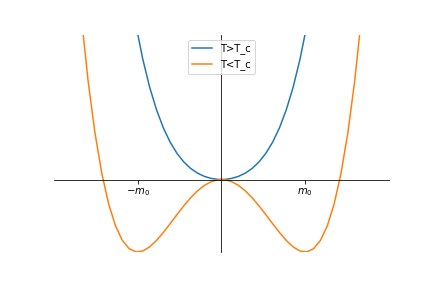
\includegraphics[width=0.7\linewidth]{landau}
	\caption{}
	\label{fig:landau}
\end{figure}

This Free Energy give rise to the familiar "Mexican Hat" of the Landau Theory of symmetry breaking.
We conclude that:
\begin{enumerate}
	\item When $T<T_c$ two different ground states appear with a non-zero magnetization
	\item The time it takes to
\end{enumerate}

\subsection{The QC mapping}




\section{Symmetry Breaking in the Quantum Ising Model}
From now on $J=1/2$ and the interaction is on the x direction:
\begin{equation}
	H_{IM}=-\frac{1}{2} \sum_{l}\left(\sigma_{l}^{x} \sigma_{l+1}^{x}+\lambda\sigma_{l}^{z}\right)
\end{equation}
This system as a spin-flip ($\mathbb{Z}_2$)	symmetry in the x direction, formally:
\begin{equation}
	[H,\otimes_i \sigma^z_i]=0
\end{equation}
If we set $\lambda=0$, the Hamiltonian \underline{in the x basis} becomes:
\begin{equation}
	H_{IM}=-\frac{1}{2} \bigoplus_l \left[\begin{array}{cccc}
		1 & 0 & 0 & 0 \\
		0 & -1 & 0 & 0 \\
		0 & 0 & -1 & 0 \\
		0 & 0 & 0 & 1 \\
	\end{array}\right]
\end{equation}
The eigenvectors with the lowest eigenvalue have the form:
\begin{equation}
	\ket{\psi_0}=\alpha\prod_i\ket{\rightarrow}_i + \beta\prod_i\ket{\leftarrow}_i
\end{equation}
The only one who respects the $\mathbb{Z}_2$ symmetry is the GHZ state:
\begin{equation}
	\ket{GHZ}=\frac{1}{\sqrt{2}}\prod_i\ket{\rightarrow}_i +\frac{1}{\sqrt{2}} \prod_i\ket{\leftarrow}_i
\end{equation}
For $\lambda>>1$ instead the ground state is simply:
\begin{equation}
	\ket{\psi_p}=\prod_i\ket{\uparrow}_i = \prod_i\frac{1}{\sqrt{2}}\left(\ket{\rightarrow}_i+\ket{\leftarrow}_i\right)
\end{equation}
\textbf{Question:} Why in the real word (and in computer simulations) we don't observe the GHZ state 
 
\appendix
\section{Mean field Approximation}\label{MFA}
The MFA for the Ising Model it's also called Bragg-Williams Approximation, it's a crude way to simplify the Ising Hamiltonian but it's qualitatively correct in 2D
\begin{equation}
	s_i =  \left\langle s_{i}\right\rangle +\delta s_i 
\end{equation} 
We neglect the quadratic corrections in $\delta s$:
\begin{equation}
	s_{i} s_{j} \simeq \left\langle s_{i}\right\rangle\left\langle s_{j}\right\rangle+\left\langle s_{j}\right\rangle \delta s_{i}+\left\langle s_{i}\right\rangle \delta s_{j}
\end{equation}
The expectation value $\left\langle s_{i}\right\rangle=m$ for every site because the system is translationally invariant.\\
Consider the Hamiltonian \ref{eq:hamiltclass} with $h=0$:
\begin{equation}
	H_{CI}=-J\sum _{\langle i~j\rangle }s _{i}s _{j}
\end{equation}
If we apply the Mean Field Approximation:
\begin{equation}
	\mathcal{H}_{MF}=-J m \sum_{\langle i j\rangle}\left(s_{i}+s_{j}-m\right)
\end{equation}
In the 2D square-lattice every site has 4 nearest-neighbors, we sum to all the $N$ sites and  divide by two to avoid double-counting:
\begin{equation}
	\mathcal{H}_{MF}=-2 J m \sum_{i=1}^{N}\left(2 s_{i}-m\right) =2N J m^{2}-4 J m \sum_{i=1}^{N} s_i
\end{equation}  
With this Hamiltonian it's quite easy to calculate the partition function:
\begin{equation}
	Z_{MF} =\operatorname{Tr}\left(e^{-\beta \mathcal{H}_{MF}}\right) 
	=\prod_{i=1}^{N}\left(\sum_{s_{i}=\pm 1}\right) e^{-\beta \mathcal{H}_{MF}}=e^{-2 \beta N  J m^{2}}\left[2 \cosh \left(4 \beta Jm\right)\right]^{N}
\end{equation}
And from there the Free Energy:
\begin{equation}
	F_{MF}=-k_B T\ln Z_{MF}=2 N  J m^{2}-N k_B T\ln 2-N k_B T \ln \left[ \cosh \beta  4Jm \right]
\end{equation}
Expanding in powers of the mean-magnetization $m$ and defining $k_{\mathrm{B}} T_{c} \equiv 4 J$ we obtain:
\begin{equation}
	f(m)=\frac{F_{MF}}{N} \simeq F_{0}+\frac{k_BT_c}{2T}\left(T-T_{c}\right) m^{2}+\frac{k_BT_c^4}{12T^3} m^{4}= F_{0}+a(T)\left(T-T_{c}\right) m^{2}+b(T) m^{4}
\end{equation}
\bibliographystyle{alpha}
\bibliography{bibanalitic}

\end{document}